%% Author: Leighton Pritchard
%% Copyright: James Hutton Institute
%% 2014-11-21: Slides for teaching at University of Strathclyde, 21st November 2014
%% This presentation was an invited guest lecture on microbial genomics and bioinformatics
%% for the BM405 course.

%% UNCOMMENT FOR SLIDES
\documentclass[table]{beamer}
\mode<presentation>

%% UNCOMMENT FOR HANDOUTS
%\documentclass[handout]{beamer}
\usepackage{handoutWithNotes}
\pgfpagesuselayout{4 on 1 with notes}[a4paper,border shrink=5mm]

%% GENERIC STYLE SETTINGS BELOW
\usetheme{default}
\usepackage{listings}
\usepackage{multirow}
\usepackage{xcolor}
\usepackage{hyperref}

\usebackgroundtemplate{

\includegraphics[width=\paperwidth,height=\paperheight]{images/hutton_background}
}
%% PRESENTATION CONFIGURATION PARAMETERS %%%%%%%%%%%%%%%%%%%%%%%%%%%%%%%%%%%%%%%
%\titlebackgroundfile{images/hutton_title}
%\framebackgroundfile{images/hutton_background}
\definecolor{hutton_green}{HTML}{78A22F}
\definecolor{hutton_purple}{HTML}{872175}
\definecolor{hutton_blue}{HTML}{569BBE}
\usefonttheme{structurebold}
\setbeamercolor{alerted text}{fg=orange}
\setbeamercolor{background canvas}{bg=white}
\setbeamercolor{block title}{bg=hutton_purple}
\setbeamercolor{frametitle}{fg=hutton_purple}
\setbeamercolor{title}{fg=black}
\setbeamercolor{titlelike}{fg=hutton_green}
\setbeamercolor{author}{fg=hutton_purple}
\setbeamercolor{author in head/foot}{fg=white}
\setbeamercolor{title in head/foot}{fg=white}
\setbeamercolor{section in head/foot}{fg=hutton_purple}
\setbeamercolor{normal text}{fg=black}
\setbeamercolor{frametitle}{fg=hutton_purple}
\setbeamerfont{block title}{size={}}
\setbeamerfont{author}{size=\footnotesize}
\setbeamerfont{institute}{size=\tiny}
\setbeamerfont{date}{size=\footnotesize}
\setbeamercolor{section in toc shaded}{fg=hutton_purple}
\setbeamercolor{section in toc}{fg=hutton_purple}
\setbeamercolor{subsection in toc shaded}{fg=hutton_purple}
\setbeamercolor{subsection in toc}{fg=hutton_purple}
\setbeamertemplate{itemize item}[circle]
\setbeamertemplate{itemize subitem}[circle]
\setbeamertemplate{itemize subsubitem}[circle]
\setbeamertemplate{itemize subsubsubitem}[circle]
\setbeamercolor{itemize item}{fg=hutton_purple}
\setbeamercolor{itemize subitem}{fg=hutton_purple}
\setbeamercolor{itemize subsubitem}{fg=hutton_purple}
\setbeamercolor{itemize subsubsubitem}{fg=hutton_purple}
\setbeamercolor{enumerate item}{fg=hutton_purple}
\setbeamercolor{enumerate subitem}{fg=hutton_purple}
\setbeamercolor{enumerate subsubitem}{fg=hutton_purple}
\setbeamercolor{enumerate subsubsubitem}{fg=hutton_purple}
\setbeamercolor{alerted text}{fg=hutton_green}
\setbeamerfont{alerted text}{series=\bfseries}
% This command makes sure that acrobat reader doesn't change the colours of the slide
% when there are figures with transparencies.
\pdfpageattr {/Group << /S /Transparency /I true /CS /DeviceRGB>>}

%Disables discrete bottom navigation bar
%\beamertemplatenavigationsymbolsempty

% Modify the slide titles to avoid the corner images,
\setbeamertemplate{frametitle}
{
\vspace{0.05\textheight}
\noindent\quad\begin{minipage}[t][0.12\textheight][t]{0.85\textwidth}
\insertframetitle\par
\end{minipage}
}

% Modify title page to avoid the big logo on right
\setbeamertemplate{title page}{
    \begin{picture}(0,0)
            %This ends up on top of the default background image, rather than replacing it:
            \put(-30,-165){%
                
\includegraphics[width=\paperwidth,height=\paperheight]{images/hutton_title}
            }
            \put(0,-75){%
                \begin{minipage}[b][0.4\textheight][t]{0.75\textwidth}
                    \usebeamerfont{title}\usebeamercolor[fg]{title}{\inserttitle\par}
                    \usebeamerfont{subtitle}\usebeamercolor[fg]{subtitle}{\insertsubtitle\par}
                \end{minipage}
            }
            \put(0,-125){%
                \begin{minipage}[b][0.1\textheight][t]{\textwidth}
                    \usebeamerfont{author}\usebeamercolor[fg]{author}{\insertauthor\par}
                    \usebeamerfont{institute}\usebeamercolor[fg]{institute}{\insertinstitute\par}
                \end{minipage}
            }
    \end{picture}
}

%%%%%%%%%%%%%%%%%%%%%%%%%%%%%%%%%%%%%%%%%%%%%%%%%%%%%%%%%%%%%%%%%%%%%%%%%%%%%%%%

% LISTINGS SETTING
% Settings for code listings in lstlistings

\definecolor{hutton_lightgreen}{HTML}{C8F27F}

\lstset{ %
  backgroundcolor=\color{hutton_lightgreen},   % choose the background color; you must add \usepackage{color} or \usepackage{xcolor}
  basicstyle=\tiny\ttfamily,        % the size of the fonts that are used for the code
  breakatwhitespace=false,         % sets if automatic breaks should only happen at whitespace
  breaklines=true,                 % sets automatic line breaking
  captionpos=b,                    % sets the caption-position to bottom
  commentstyle=\color{red},    % comment style
  deletekeywords={...},            % if you want to delete keywords from the given language
  escapeinside={\%*}{*)},          % if you want to add LaTeX within your code
  extendedchars=true,              % lets you use non-ASCII characters; for 8-bits encodings only, does not work with UTF-8
  frame=single,                    % adds a frame around the code
  keepspaces=true,                 % keeps spaces in text, useful for keeping indentation of code (possibly needs columns=flexible)
  keywordstyle=\color{blue},       % keyword style
%  language=Octave,                 % the language of the code
  morekeywords={*,...},            % if you want to add more keywords to the set
  numbers=left,                    % where to put the line-numbers; possible values are (none, left, right)
  numbersep=5pt,                   % how far the line-numbers are from the code
  numberstyle=\tiny\color{gray}, % the style that is used for the line-numbers
  rulecolor=\color{black},         % if not set, the frame-color may be changed on line-breaks within not-black text (e.g. comments (green here))
  showspaces=false,                % show spaces everywhere adding particular underscores; it overrides 'showstringspaces'
  showstringspaces=false,          % underline spaces within strings only
  showtabs=false,                  % show tabs within strings adding particular underscores
  stepnumber=1,                    % the step between two line-numbers. If it's 1, each line will be numbered
  stringstyle=\color{violet},     % string literal style
  tabsize=4,                       % sets default tabsize to 2 spaces
  title=\lstname                   % show the filename of files included with \lstinputlisting; also try caption instead of title
}


%%%
% TITLE PREAMBLE
\title[Microbial Genomics and Bioinformatics: 4.Genome Features] % (optional, only for long titles)
{Microbial Genomics and \\ Bioinformatics \\
BM405 \\
4.Genome Features}
%\subtitle{}
\author[Pritchard] % (optional, for multiple authors)
{Leighton~Pritchard$^{1,2,3}$}
\institute[The James Hutton Institute] % (optional)
{
  $^{1}$Information and Computational Sciences,\\
  $^{2}$Centre for Human and Animal Pathogens in the Environment,\\
  $^{3}$Dundee Effector Consortium,\\
  The James Hutton Institute, Invergowrie, Dundee, Scotland, DD2 5DA
}
\date[21st November 2014] % (optional)
{21st November 2014}
\subject{Bioinformatics, Genomics, Bacteria, Sequencing, Microbiology, Microbes}

%%%
% TOC
% Show table of contents, with current section highlighted,
% at the start of each section

%\AtBeginSection[]
%{
%  \begin{frame}
%    \frametitle{Table of Contents}
%    \tableofcontents[currentsection] %,hideallsubsections]
%  \end{frame}
%}

\AtBeginSubsection[]
{
  \begin{frame}
    \frametitle{Table of Contents}
    \tableofcontents[currentsection,currentsubsection] %,hideallsubsections]
  \end{frame}
}

%%%
% START DOCUMENT
\begin{document}

\frame[plain]{\titlepage}

%% use.tex
%% Author: Leighton Pritchard
%% Copyright: James Hutton Institute
%% These slides describe the acceptable use policy for these slides and
%% materials

%
\begin{frame}
  \frametitle{Acceptable Use Policy}
  Recording of this talk, taking photos, discussing the content using \\
  email, Twitter, blogs, etc. is permitted (and encouraged), \\
  providing distraction to others is minimised. \\[0.5cm]
  These slides will be made available on SlideShare. \\[0.5cm]
  These slides, and supporting material, are available at \href{https://github.com/widdowquinn/Teaching-2014-11-21-Strathclyde}{https://github.com/widdowquinn/Teaching-2014-11-21-Strathclyde}
\end{frame}

%%%
% SECTION: Genome features
\section{Genome Features}
%% genome_features.tex
%% Author: Leighton Pritchard
%% Copyright: James Hutton Institute
%% A brief description of genome feature prediction, and related
%% issues


% SUBSECTION: Genome Features
\subsection{What are genome features?}

% What do you align, and why?
\begin{frame}
  \frametitle{Genome Features}
  \begin{itemize}
    \item Genome features are annotated regions of the genome.
    \item Typically represent functional elements.
    \item May be simple (single region), or complex (subfeatures)
  \end{itemize}
\end{frame}

% Gene features
\begin{frame}
  \frametitle{Gene Features}
  Gene features have significant substructure, especially in eukaryotes.
  \begin{columns}[T]
    \begin{column}{4cm}
      \begin{itemize}
      \item 5` UTR
        \item translation start
        \item intron start/stop
        \item exon start/stop
        \item translation stop
        \item translation terminator
        \item 3` UTR
      \end{itemize}
    \end{column}
    \begin{column}{6cm}
      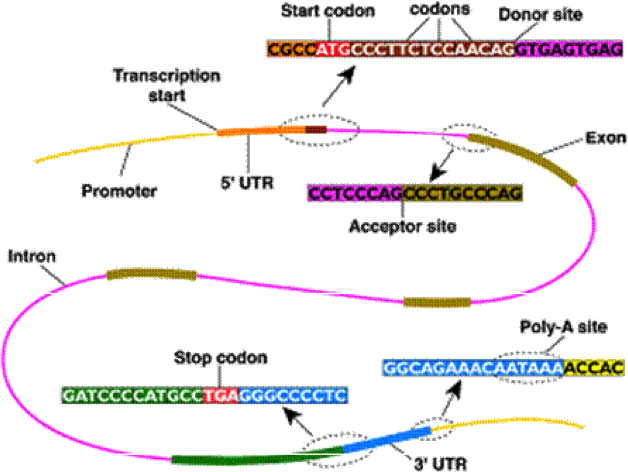
\includegraphics[width=1\textwidth]{images/eukaryotic_gene}
    \end{column}
  \end{columns}       
\end{frame}

% ncRNA features
\begin{frame}
  \frametitle{ncRNA Features}
  \begin{columns}[T]
    \begin{column}{5cm}
      \begin{itemize}
        \item tRNA - transfer RNA
        \item rRNA - ribosomal RNA
        \item CRISPRs - bacterial/archaeal defence (used for genome editing)
        \item many other classes
      \end{itemize}
    \end{column}
    \begin{column}{5cm}
      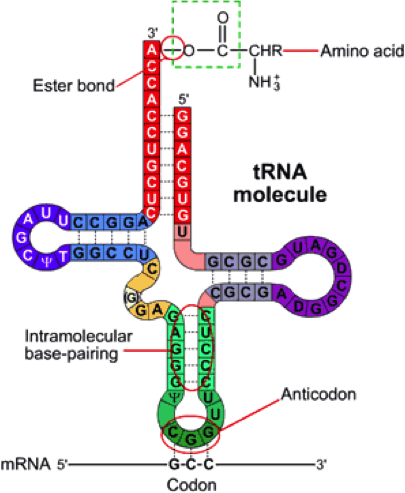
\includegraphics[width=1\textwidth]{images/ncrna}
    \end{column}
  \end{columns}       
\end{frame}

% Regulatory features
\begin{frame}
  \frametitle{Regulatory/Repeat Features}
  \textbf{Regulatory sites}
  \begin{itemize}
    \item transcription start sites
    \item RNA polymerase binding sites
    \item Transcription Factor Binding Sites (TFBS)
  \end{itemize}
  \begin{center}
    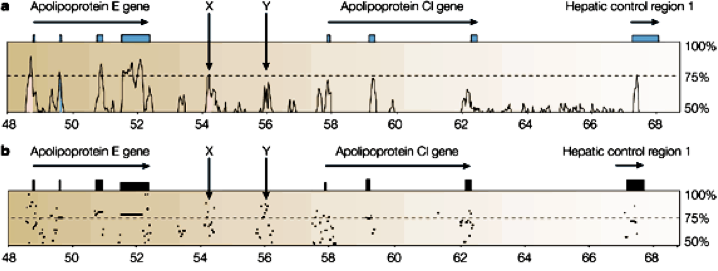
\includegraphics[width=0.5\textwidth]{images/regulatory_sites}
  \end{center}
  \textbf{Repetitive regions and mobile elements}
  \begin{itemize}
    \item tandem repeats
    \item (retro-)transposable elements
    \item phage inclusions
  \end{itemize}  
\end{frame}

% Principles of feature prediction
\begin{frame}
  \frametitle{Principles of feature prediction}
  Two main approaches to feature prediction:
  \begin{itemize}
    \item \textit{ab initio} prediction - start from first principles, using only the genome sequence: 
    \begin{itemize}
      \item Unsupervised methods - not trained on a dataset
      \item Supervised methods - trained on a dataset
    \end{itemize}
    \item homology matches
    \begin{itemize}
      \item alignment to features from related organisms (comparative genomics, annotation transfer)
      \item from known gene products (e.g. proteins, ncRNA)
      \item from transcripts/other intermediates (e.g. ESTs, cDNA, RNAseq)
    \end{itemize}
  \end{itemize}
  Dedicated tools available for many different classes of feature.
\end{frame}
%% gene_prediction.tex
%% Author: Leighton Pritchard
%% Copyright: James Hutton Institute
%% A brief description of gene prediction, as an illustrative example

% SUBSECTION: Prokaryotic CDS prediction
\subsection{Prokaryotic CDS Prediction}

% Prokaryotic gene prediction
\begin{frame}
  \frametitle{Prokaryotic CDS Prediction Methods}
  Using CDS prediction as an illustrative example for all feature prediction.\\[0.2cm]
  \begin{itemize}
    \item Prokaryotes ``easier'' than eukaryotes for gene/CDS prediction
    \item Less uncertainty in predictions (isoforms, gene structure)
    \begin{itemize}
      \item Very gene-dense (over 90\% of chromosome is coding sequence)
      \item No intron-exon structure
      \item Problem is: ``which possible ORF contains the true gene, and which start site is correct?''
      \item Still not a solved problem
    \end{itemize}       
  \end{itemize}
\end{frame}

% Finding ORFs
\begin{frame}
  \frametitle{Finding Open Reading Frames}
  The simplest approach: find ORFs (sequence between two consecutive in-frame stop codons)
  \begin{itemize}
    \item<1-> ORF finding is naive, does not consider:
    \begin{itemize}
      \item Start codon
      \item Promoter/RBS motifs
      \item Wider context (e.g. overlapping genes)
    \end{itemize}
  \end{itemize}
  Dedicated tools, e.g. \texttt{Glimmer}, \texttt{Prodigal}, \texttt{RAST}, \texttt{GeneMarkS} usually better.
\end{frame}

% Two alternative methods
\begin{frame}
  \frametitle{Two \textit{ab initio} Prokaryotic Prediction Tools}
  \begin{itemize}
    \item \texttt{Glimmer}\footnote{\tiny{\href{http://dx.doi.org/10.1093/bioinformatics/btm009}{Delcher \textit{et al}. (2007) \textit{Bioinformatics} \textbf{23}:673-679 doi:10.1093/bioinformatics/btm009}}}
    \begin{itemize}
      \item Interpolated Markov models
      \item Can be trained on ``gold standard'' datasets
    \end{itemize}
    \item \texttt{Prodigal}\footnote{\tiny{\href{http://dx.doi.org/10.1186/1471-2105-11-119}{Hyatt \textit{et al}. (2010) \textit{BMC Bioinf.} \textbf{11}:119 doi:10.1186/1471-2105-11-119}}}
    \begin{itemize}
      \item Log-likelihood model based on GC frame plots, followed by dynamic programming
      \item Can be trained on ``gold standard'' datasets
    \end{itemize}
  \end{itemize}
  Applying these to an example bacterial chromosome$\ldots$
\end{frame}

\begin{frame}
  \frametitle{Comparing predictions in Artemis\footnote{\tiny{\href{http://dx.doi.org/10.1093/bioinformatics/btr703}{Carver \textit{et al}. (2012) \textit{Bioinformatics} \textbf{28}:464-469 doi:10.1093/bioinformatics/btr703}}}}
  Not every ORF (green) is predicted to encode for a coding sequence (CDS; blue/orange).\\
  Self-contradictory CDS calls (orange); even automated annotation needs manual curation.
  \begin{center}
    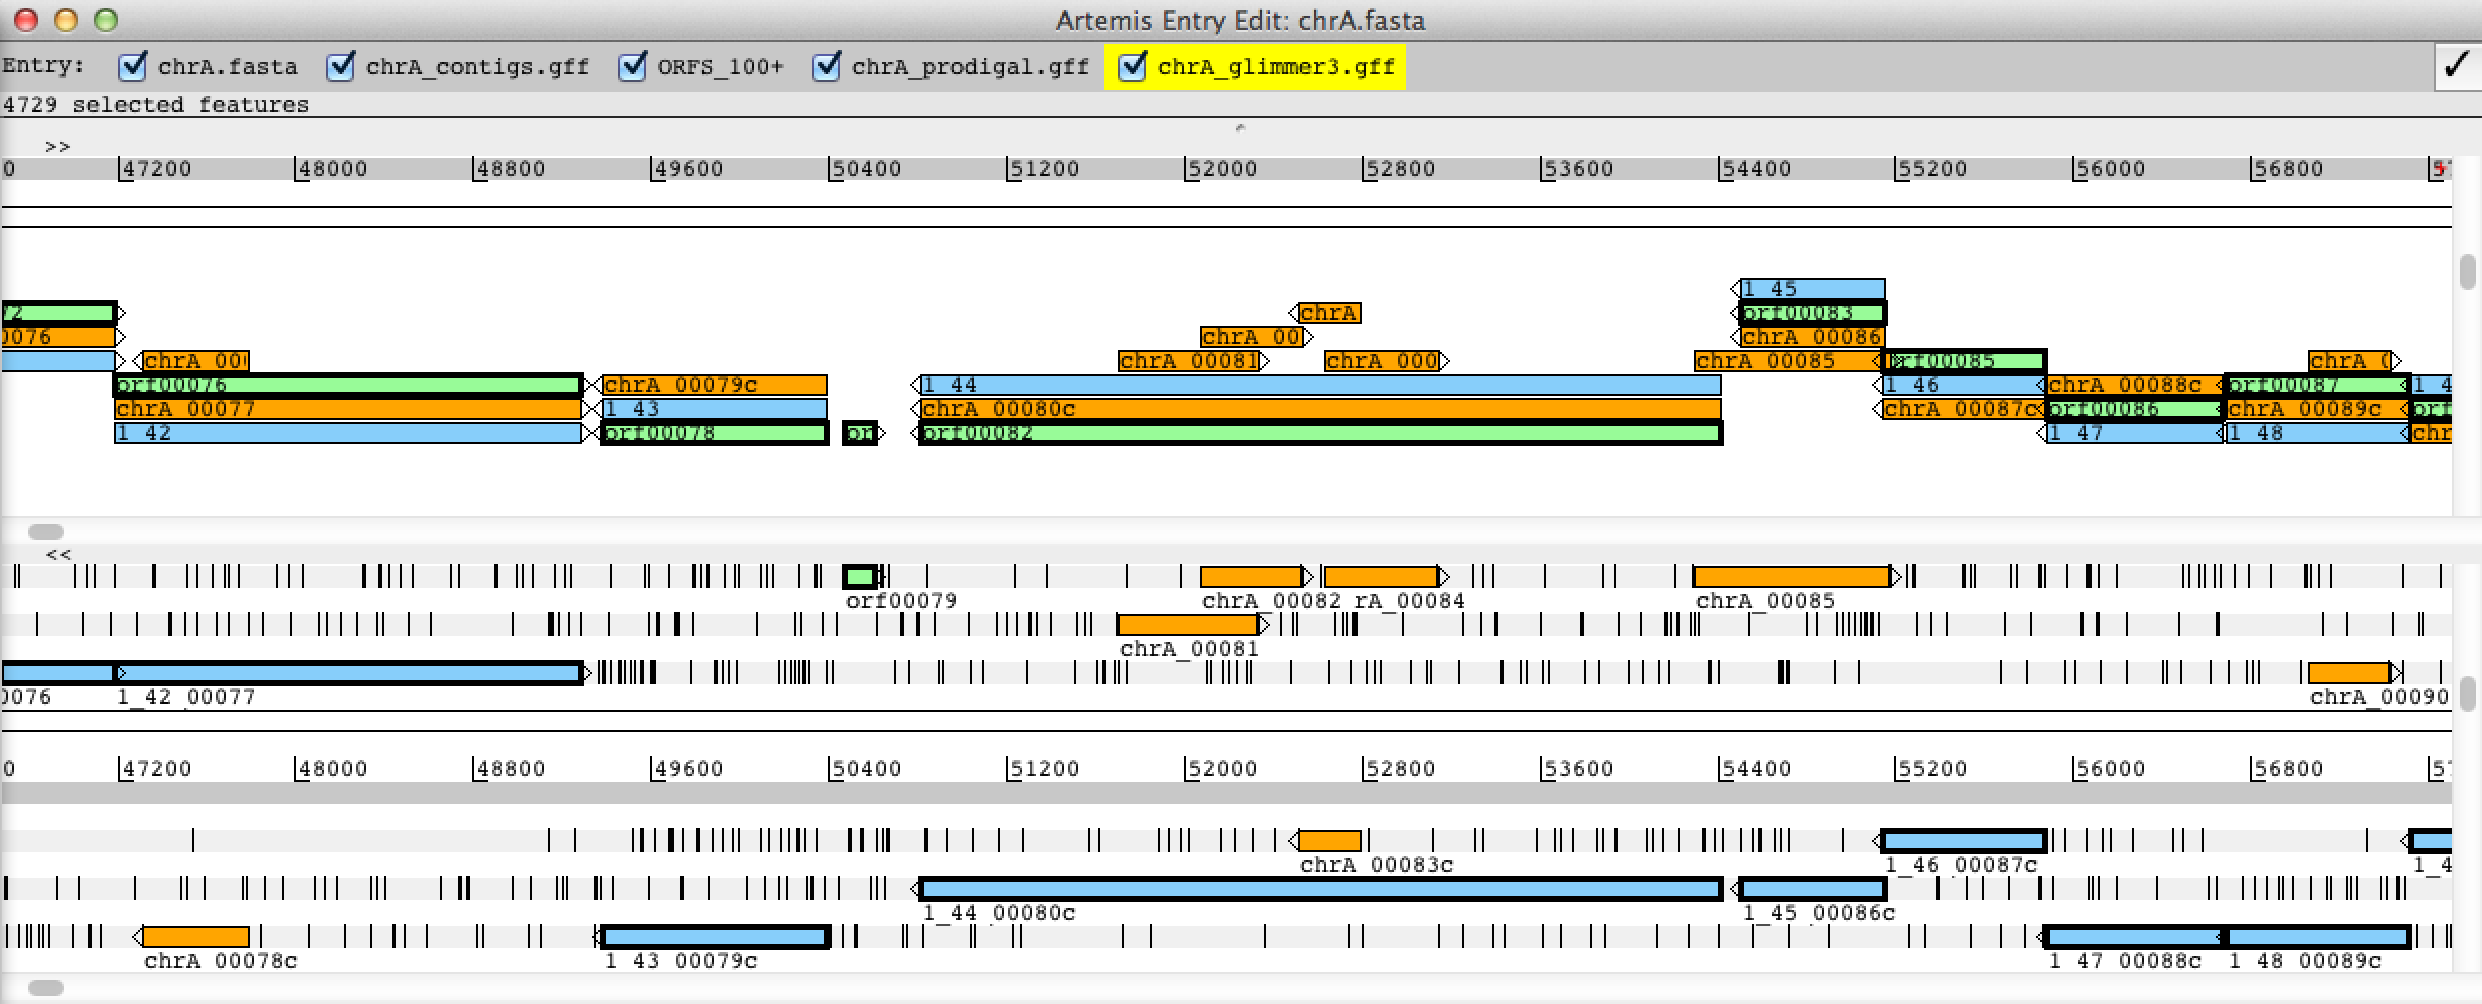
\includegraphics[width=1\textwidth]{images/artemis_cdspred3}     
  \end{center}
\end{frame}

\begin{frame}
  \frametitle{Comparing predictions in Artemis}
  \texttt{Glimmer}(green)/\texttt{Prodigal}(blue) CDS prediction methods do not always agree.
  \begin{center}
    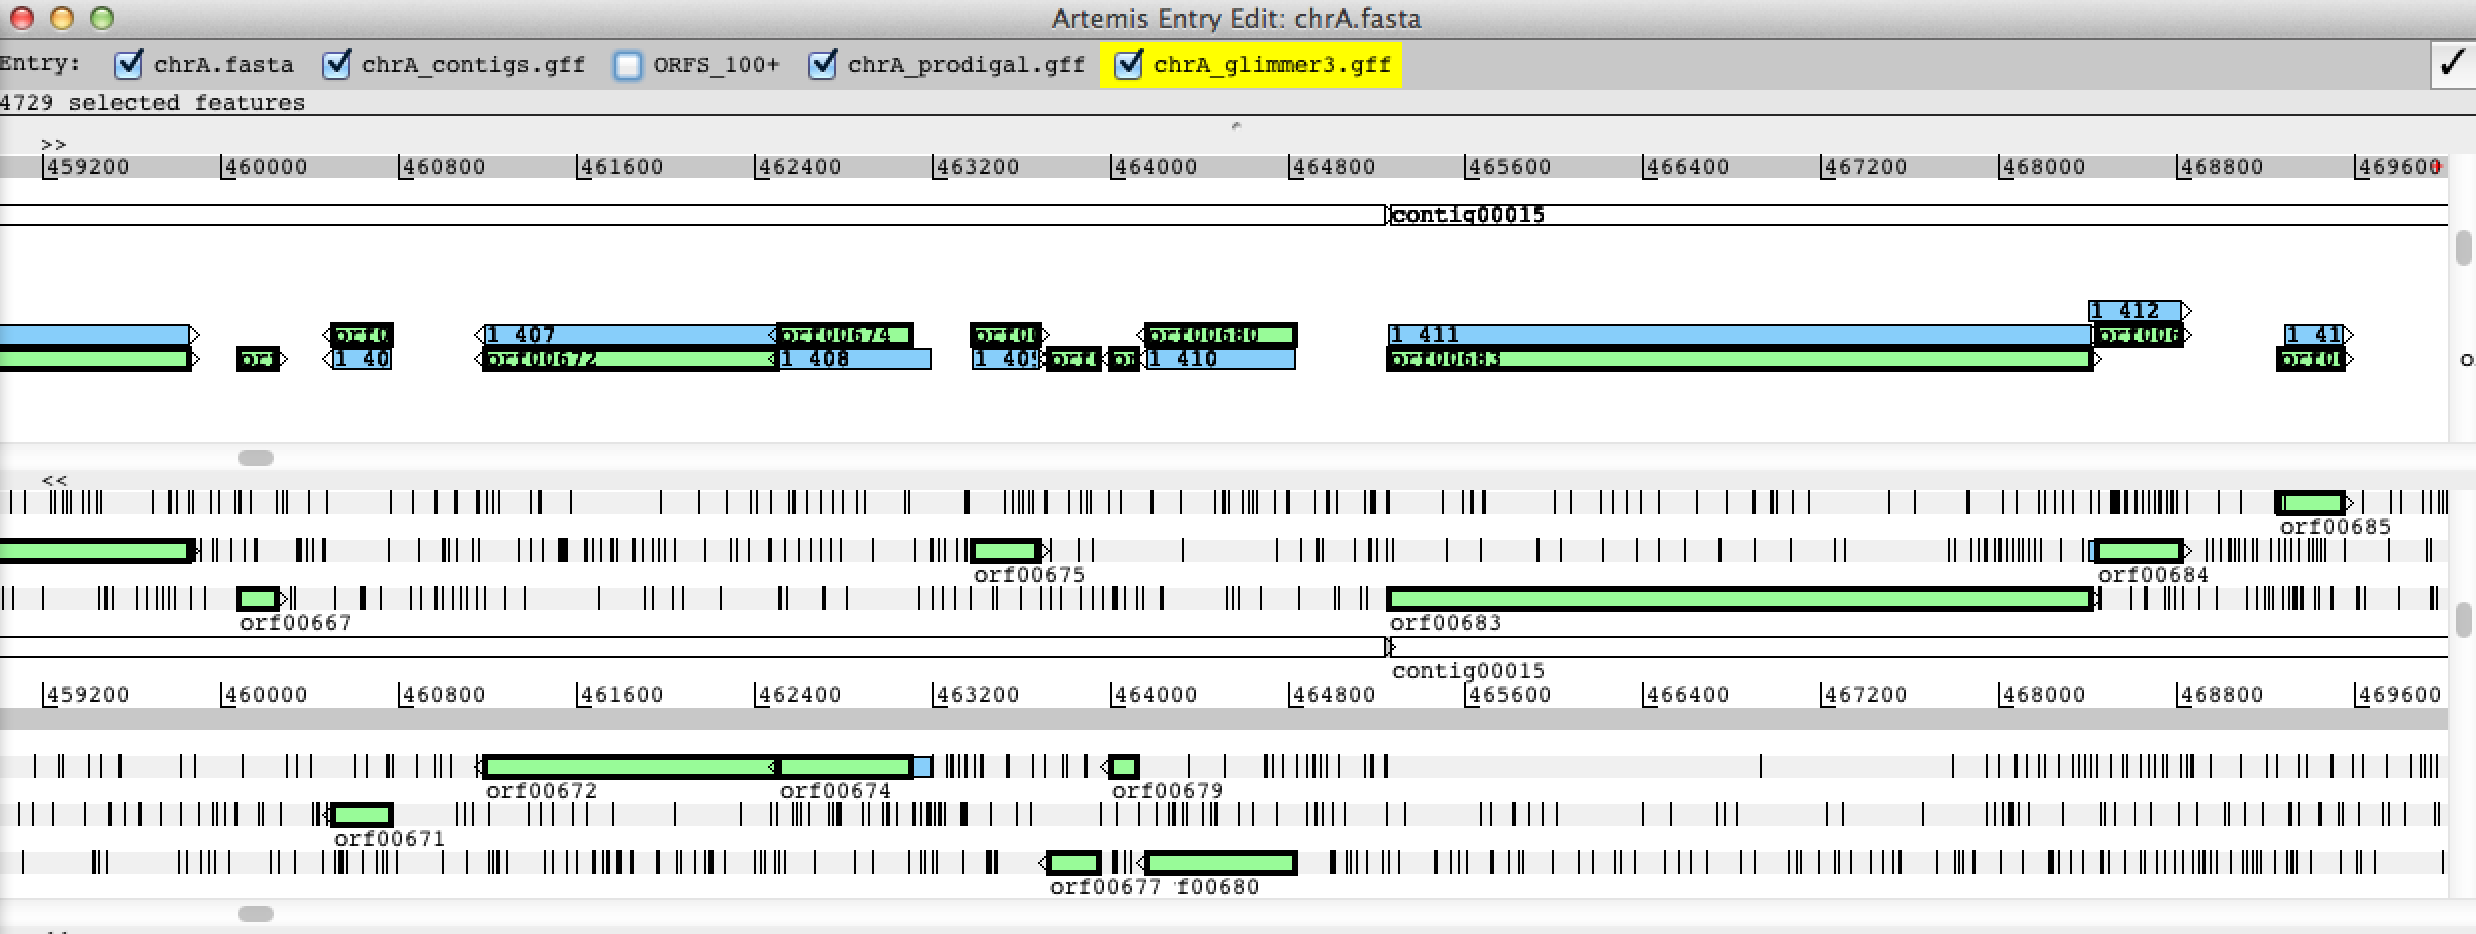
\includegraphics[width=1\textwidth]{images/artemis_cdspred4}     
  \end{center}
  How do we know which (if either) is best?
\end{frame}
%% assessing_gene_prediction.tex
%% Author: Leighton Pritchard
%% Copyright: James Hutton Institute
%% A brief description of gene prediction, as an illustrative example

% SUBSECTION: Assessing Prediction Methods
\subsection{Assessing Prediction Methods}

% Method validation
\begin{frame}
  \frametitle{Using a ``Gold Standard'': validation\footnote{\tiny{\href{http://dx.doi.org/10.1007/978-1-62703-986-4_4}{Pritchard and Broadhurst (2014) \textit{Methods Mol. Biol.} \textbf{1127}:53-64 doi:10.1007/978-1-62703-986-4\_4}}}}
  A general approach for \emph{all} predictive methods
  \begin{itemize}
    \item Define a known, ``correct'' set of true/false, positive/negative etc. examples - the ``gold standard''
    \item Evaluate your predictive method against that set for
    \begin{itemize}
      \item sensitivity, specificity, accuracy, precision, etc.
    \end{itemize}
  \end{itemize}
  This ought to be done by the method developers, but often wise to evaluate in your own system.\\[0.1cm]
  Many methods available, coverage beyond the scope of this introduction
\end{frame}

% Contingency tables and performance metrics
\begin{frame}
  \frametitle{Contingency Tables}
  \begin{center}
     \begin{tabular}{cc|c|c|}
	  \cline{3-4}
		& & \multicolumn{2}{|c|}{Condition (Gold standard)}\\
	  \cline{3-4}
		& & True & False \\
	  \hline
	  \multicolumn{1}{ |c| }{\multirow{2}{*}{Test outcome}}& 
	  %\multicolumn{1}{ |c| }{Positive} & True Positive \cellcolor{green} & 
	  %  False Positive\cellcolor{red}\\
	  \multicolumn{1}{ |c| }{Positive} & True Positive  & 
	    False Positive\\
	  \cline{2-4}
	  \multicolumn{1}{ |c| }{} & \multicolumn{1}{ |c| }{Negative} & 
	    %False Negative\cellcolor{red} & True Negative \cellcolor{green}\\
	    False Negative & True Negative \\
	  \hline
    \end{tabular}
  \end{center}
  \textbf{Performance Metrics}\\
  Sensitivity = TPR = $TP/(TP + FN)$ \\
  Specificity = TNR = $TN/(FP + TN)$ \\
  FPR = $1-\text{Specificity} = FP/(FP + TN)$ \\[0.1cm]
  \textbf{If you don't have this information, you can't interpret predictive results properly.}
\end{frame}

% Testing CDS prediction on gold standards
\begin{frame}
  \frametitle{``Gold Standard'' results}
  \begin{itemize}
    \item Tested \texttt{glimmer}\footnote{\tiny{\href{http://dx.doi.org/10.1093/bioinformatics/btm009}{Delcher \textit{et al}. (2007) \textit{Bioinformatics} \textbf{23}:673-679 doi:10.1093/bioinformatics/btm009}}} and \texttt{prodigal}\footnote{\tiny{\href{http://dx.doi.org/10.1186/1471-2105-11-119}{Hyatt \textit{et al}. (2010) \textit{BMC Bioinf.} \textbf{11}:119 doi:10.1186/1471-2105-11-119}}} on two enterobacterial close relatives as "gold standards"
    \begin{itemize}
      \item Manually annotated ($>$3 expert person years)
      \item Community-annotated (many research groups, interested in their own subset of genes)
    \end{itemize}
    \item \textbf{Both methods trained directly on the annotated genes in each organism!}
  \end{itemize} 
\end{frame}

% Test on manually annotated set
\begin{frame}
  \frametitle{``Gold Standard'' results}
  \textbf{Manually annotated}: 4550 CDS
  \begin{center}
    \begin{tabular}{r|l|l}
	  genecaller & \texttt{glimmer} & \texttt{prodigal}  \\
	  \hline
	  predicted & 4752    & 4287  \\
	  missed & \textbf{284} (6\%)   & 407 (9\%)  \\
	  \hline
	  \emph{Exact Prediction} & & \\
  	  sensitivity   & 62\%   & \textbf{71}\%  \\
  	  FDR   & 41\%   & \textbf{25}\%  \\  
	  PPV   & 59\% & \textbf{75}\%  \\  
	  \hline
	  \emph{Correct ORF} & & \\
  	  sensitivity   & \textbf{94}\%   & 91\% \\
  	  FDR   & 10\%  & \textbf{3}\% \\  
	  PPV   & 90\% & \textbf{97}\%  \\  
    \end{tabular}
  \end{center}     
\end{frame}

% Test on community annotated set
\begin{frame}
  \frametitle{``Gold Standard'' results}
  \textbf{Community annotated}: 4475 CDS
  \begin{center}
	\begin{tabular}{r|l|l}
	  genecaller & \texttt{glimmer} & \texttt{prodigal}  \\
	  \hline
	  predicted & 4679    & 4467  \\
	  missed & \textbf{112} (3\%)   & 156 (3\%)  \\
	  \hline
	  \emph{Exact Prediction} & & \\
  	  sensitivity   & 62\%   & \textbf{86}\%  \\
  	  FDR   & 31\%   & \textbf{14}\%  \\  
	  PPV   & 69\% & \textbf{86}\%  \\  
	  \hline
	  \emph{Correct ORF} & & \\
  	  sensitivity   & \textbf{97}\%   & \textbf{97}\% \\
  	  FDR   & 7\%  & \textbf{3}\% \\  
	  PPV   & 93\% & \textbf{97}\%  \\  
	\end{tabular}
  \end{center}     
\end{frame}

% Conclusions from these comparisons
\begin{frame}
   \frametitle{Gene/CDS Prediction}   
   \framesubtitle{Lessons learned}   
   \begin{itemize}
     \item Alternative CDS (and all other) prediction methods are unlikely to give identical results, or perform equally well
     \item \textbf{There is No Free Lunch} (this is a theorem: \href{http://en.wikipedia.org/wiki/No_free_lunch_theorem}{http://en.wikipedia.org/wiki/No\_free\_lunch\_theorem})
     \item To assess/choose between methods, performance metrics are required
     \item Even on (relatively simple) prokaryotes, current best methods for CDS prediction are imperfect
     \item Manual assessment and intervention is essential, and usually the most demanding and time-consuming part of the process
   \end{itemize}
\end{frame}

%% annotation_pipelines.tex
%% Author: Leighton Pritchard
%% Copyright: James Hutton Institute
%% A brief description of gene prediction, as an illustrative example

% SUBSECTION: Annotation Pipelines
\subsection{Prokaryotic Annotation Pipelines}

% Prokaryotic annotation pipelines
\begin{frame}
  \frametitle{Prokaryotic Annotation Pipelines\footnote{\tiny{\href{http://dx.doi.org/10.1093/bib/bbs007}{Richardson and Watson (2012) \textit{Brief. Bioinf.} \textbf{14}:1-12 doi:10.1093/bib/bbs007}}}}
  Many choices, including \texttt{RAST}\footnote{\tiny{\href{http://dx.doi.org/10.1186/1471-2164-9-75}{Aziz \textit{et al}. (2008) \textit{BMC Genomics} \textbf{9}:75 doi:10.1186/1471-2164-9-75}}}, \texttt{PROKKA}\footnote{\tiny{\href{http://dx.doi.org/10.1093/bioinformatics/btu153}{Seemann (2014) \textit{Bioinformatics} \textbf{30}:2068-2069 doi:10.1093/bioinformatics/btu153}}}, \texttt{BaSYS}\footnote{\tiny{\href{http://dx.doi.org/10.1093/nar/gki593}{Van Domselaar \textit{et al}. (2005) \textit{Nuc. Acids Res.} \textbf{33}:W455-W459 doi:10.1093/nar/gki593}}}, etc.\\
  Often perform both CDS/feature calling and functional prediction.\\
  Two broad approaches:
  \begin{enumerate}
    \item Heavyweight: maintain database and resource, often annotating by homology, e.g. \texttt{RAST}
    \item Lightweight: chain together multiple third-party packages, e.g. \texttt{PROKKA}
  \end{enumerate}
  Pipelines take a lot of tedium (and control) out of annotating bacterial genomes, but have the same issues as every other prediction tool.
\end{frame}

% PROKKA
\begin{frame}
  \frametitle{PROKKA\footnote{\tiny{\href{http://dx.doi.org/10.1093/bioinformatics/btu153}{Seemann (2014) \textit{Bioinformatics} \textbf{30}:2068-2069 doi:10.1093/bioinformatics/btu153}}}}
  \begin{columns}
    \begin{column}{5cm}
      \begin{itemize}
        \item Lightweight, and fast. 
        \item Runs locally. (5Mbp genome takes $\approx$10min on my desktop; more detailed ncRNA prediction takes $\approx$20min)
        \item Flexible: built-in databases can be replaced by user databases.
        \item Uses freely-accessible third-party tools for prediction
      \end{itemize}
    \end{column}
    \begin{column}{5cm}
      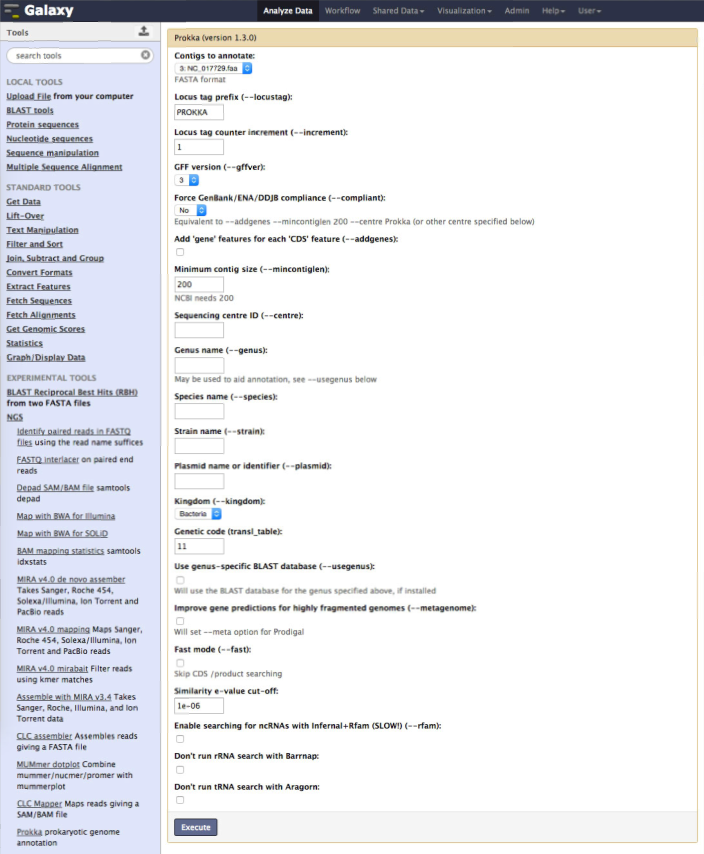
\includegraphics[width=0.9\textwidth]{images/prokka_galaxy}
    \end{column}
  \end{columns}
  Simple to run (at the command-line, or in \texttt{Galaxy}\footnote{\tiny{\href{http://dx.doi.org/10.1186/gb-2010-11-8-r86}{Goecks \textit{et al}. (2010) \textit{Genome Biol.} \textbf{11}:R86 doi:10.1186/gb-2010-11-8-r86}}}). \\
\end{frame}

% RAST
\begin{frame}
  \frametitle{RAST\footnote{\tiny{\href{http://dx.doi.org/10.1186/1471-2164-9-75}{Aziz \textit{et al}. (2008) \textit{BMC Genomics} \textbf{9}:75 doi:10.1186/1471-2164-9-75}}}}
  \begin{columns}
    \begin{column}{5cm}
      \begin{itemize}
        \item Server-based (\href{http://rast.nmpdr.org/}{http://rast.nmpdr.org/}). Queues likely.
        \item Relies on SEED and FIGFam databases, held at NMPDR
        \item \textbf{FIGFam}: isofunctional homologue families
        \item \textbf{Produces metabolic reconstruction}
      \end{itemize}
    \end{column}
    \begin{column}{5cm}
      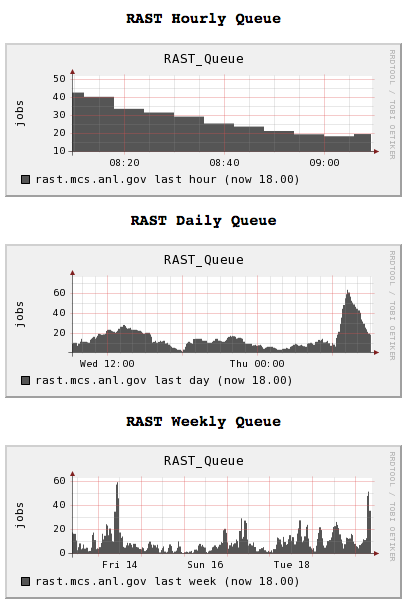
\includegraphics[width=0.9\textwidth]{images/rast_queue}
    \end{column}
  \end{columns}
\end{frame}

%%%
% SECTION: Genome-Scale Functional Prediction
\section{Genome-Scale Functional Annotation}
%% functional_annotation.tex
%% Author: Leighton Pritchard
%% Copyright: James Hutton Institute
%% A brief description of functional annotation

% SUBSECTION: Functional Annotation
\subsection{Functional Annotation}

% Principles of function prediction
\begin{frame}
  \frametitle{Principles of function prediction}
  At genome scale, we realistically have to automate function prediction. \\
  \textbf{Function prediction is just like any other prediction method.} \\
  Two main approaches to function prediction:
  \begin{itemize}
    \item \textit{ab initio} prediction (on basis of feature sequence/context only)
    \begin{itemize}
      \item Unsupervised methods - not trained on an exemplar dataset
      \item Supervised methods - trained on an exemplar dataset
    \end{itemize}
    \item homology matches (sequence similarity)
    \begin{itemize}
      \item alignment to features with known/predicted functions
    \end{itemize}
  \end{itemize}
\end{frame}

% Homology-based methods
\begin{frame}
  \frametitle{Homology-based function prediction}
  Two proteins with similar sequence may have similar function.\\
  But$\ldots$
  \begin{itemize}
    \item How similar do they have to be (and where) to share the same function?
    \item What do we mean by `same function', anyway: interaction/substrate specificity? participation in a pathway? contribution to a structure? biochemical interconversion? $\ldots$
    \item How confident can we be in the comparator (annotated) sequence: was \textit{that} function determined experimentally?
  \end{itemize}
\end{frame}

% Gene Ontology
\begin{frame}
  \frametitle{Gene Ontology (GO)\footnote{\tiny{\href{http://dx.doi.org/10.1038/75556}{Ashburner \textit{et al}. (2000) \textit{Nat. Genet.} \textbf{25}:25-29 doi:10.1038/75556}}}}
  The Gene Ontology provides a common vocabulary for describing biological function, and unifying functional descriptions.\\[0.1cm]
  \textbf{Ontologies (controlled vocabularies) are central to information-sharing.} \\[0.1cm]
  Gene Ontology Consortium: \href{http://geneontology.org/}{http://geneontology.org/} \\[0.1cm]
  Many annotation tools and databases produce GO output, or compatible controlled vocabulary terms, e.g.
  \begin{itemize}
    \item Blast2GO\footnote{\tiny{\href{http://dx.doi.org/10.1093/bioinformatics/bti610}{Conesa \textit{et al}. (2005) \textit{Bioinformatics} \textbf{21}:3674-3676 doi:10.1093/bioinformatics/bti610}}}: BLAST-based annotation
    \item PHI-Base\footnote{\tiny{\href{http://dx.doi.org/10.1093/nar/gkj047}{Winnenburg \textit{et al}. (2006) \textit{Nuc. Acids Res.} \textbf{34}:D459-D464 doi:10.1093/nar/gkj047}}}: microbial pathogen-host interaction specific functions
    \item GOPred\footnote{\tiny{\href{http://dx.doi.org/10.1371/journal.pone.0012382}{Sarac \textit{et al}. (2010) \textit{PLoS One} \textbf{5}:e12382 doi:10.1371/journal.pone.0012382}}}: combines several protein function classifiers
  \end{itemize}
\end{frame}

% Gene Ontology
\begin{frame}
  \frametitle{Gene Ontology (GO)\footnote{\tiny{\href{http://dx.doi.org/10.1038/75556}{Ashburner \textit{et al}. (2000) \textit{Nat. Genet.} \textbf{25}:25-29 doi:10.1038/75556}}}}
  \begin{center}
    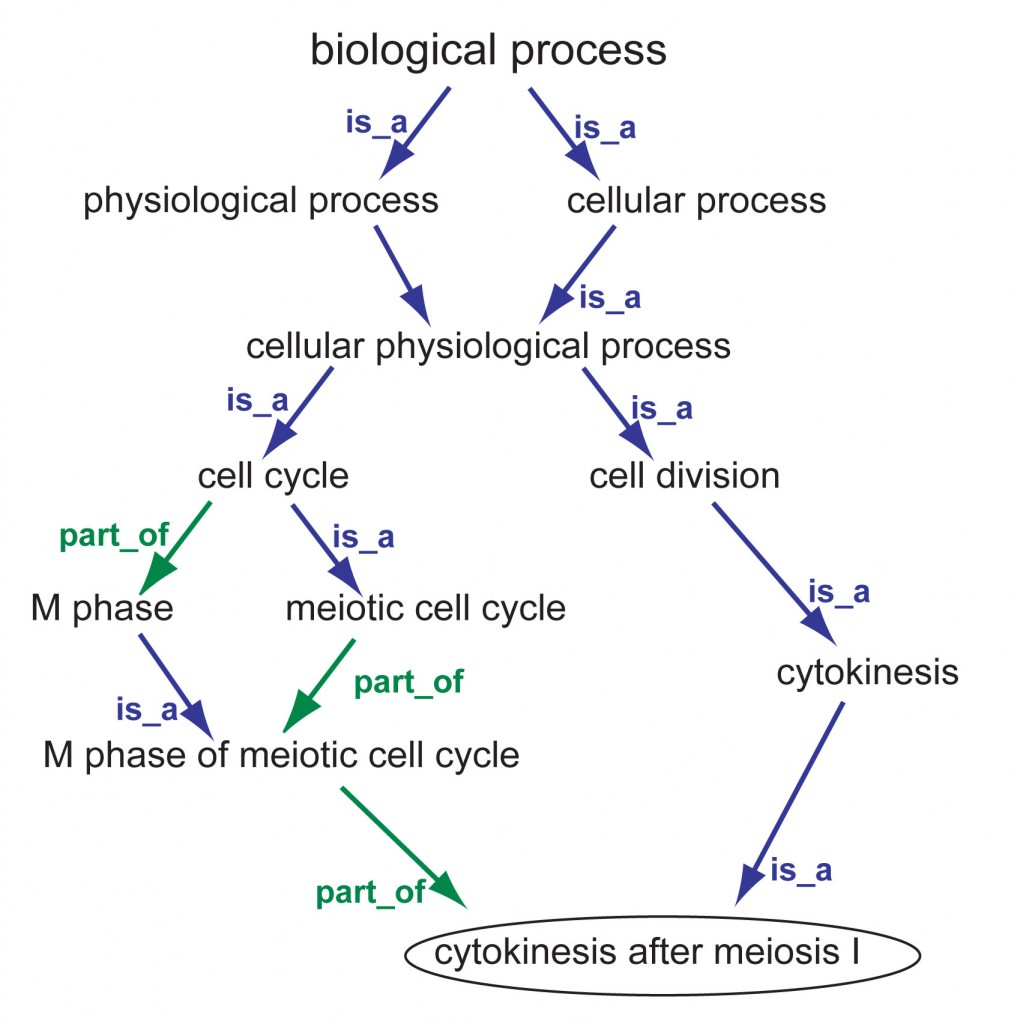
\includegraphics[height=0.7\textheight]{images/go_example}
  \end{center}
\end{frame}

% How good are database annotations?
\begin{frame}
  \frametitle{Are database annotations reliable?\footnote{\tiny{\href{http://dx.doi.org/10.1371/journal.pcbi.1003063}{Schnoes \textit{et al}. (2013) \textit{PLoS Comp. Biol.} \textbf{9}:e1003063 doi:10.1371/journal.pcbi.1003063}}}}
  Are protein function annotations in databases determined experimentally, or by annotation transfer?\\[0.1cm]
  High throughput experiments and genome annotations are conducted without validation of function, and placed in databases.\\[0.1cm]
  \begin{itemize}
    \item GO databases record annotation origin by publication 
    \item GO databases record evidence codes, e.g.: \textbf{EXP}=Inferred from Experiment; \textbf{ISS}=Inferred from Sequence Similarity
    \item 0.14\% of contributing publications provide 25\% of all experimentally validated annotations in the Uniprot-GOA compilation.
    \item There are biases in functional annotation.
  \end{itemize}
  No clear solution to this kind of bias - \textbf{but we have to recognise and account for it}.
\end{frame}

% How good are database annotations?
\begin{frame}
  \frametitle{Are database annotations reliable?\footnote{\tiny{\href{http://dx.doi.org/10.1038/nmeth.2340}{Radivojac \textit{et al}. (2013) \textit{Nat. Meth.} \textbf{10}:221-227 doi:10.1038/nmeth.2340}}}}
  The Critical Assessment of Function Annotation (CAFA) project.
  \begin{center}
    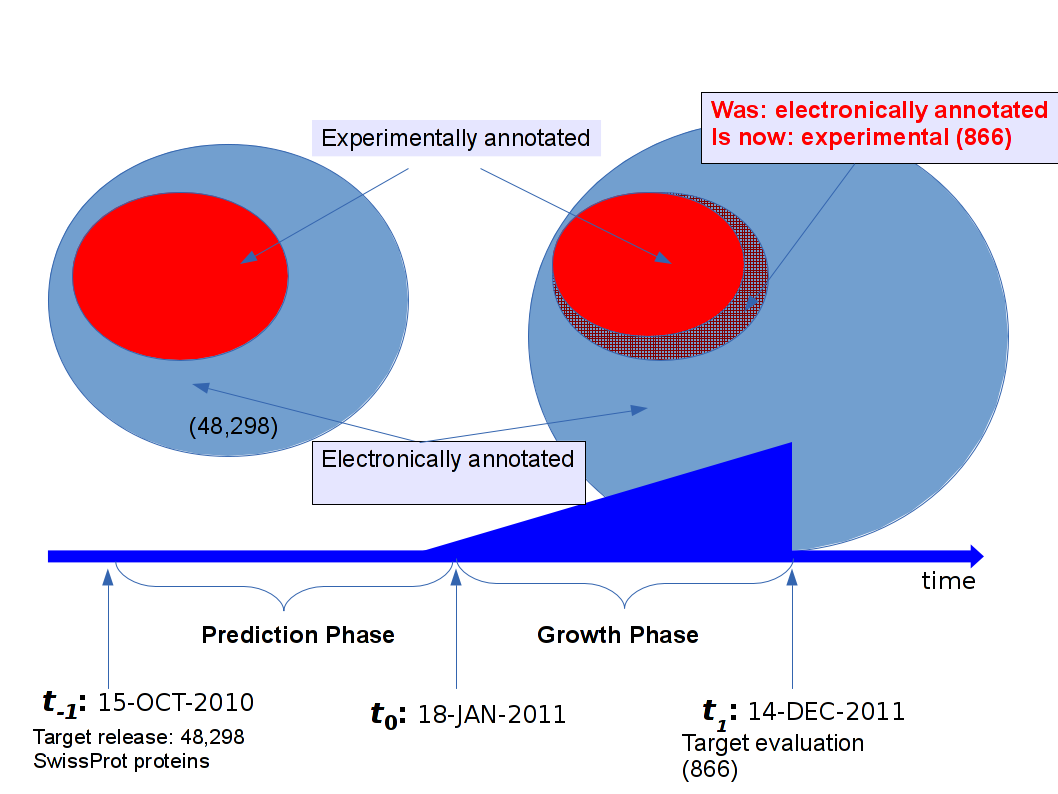
\includegraphics[height=0.7\textheight]{images/cafa_annotation_problem}
  \end{center}   
\end{frame}

% Homology-based methods
\begin{frame}
  \frametitle{Do biased database annotations matter?}
  Experimental annotations of proteins are incomplete. But is that important?\\
  Tested by simulation, and following databases for three years.\footnote{\tiny{\href{http://dx.doi.org/10.1093/bioinformatics/btu472}{Jiang \textit{et al}. (2014) \textit{Bioinformatics} \textbf{30}:i609-i616 doi:10.1093/bioinformatics/btu472}}}
  \begin{enumerate}
    \item Yes. It matters.
    \item Current large scale annotations are meaningful and almost surprisingly reliable.
    \item The nature and level of data incompleteness, and type of classification model have an effect.
    \item ``Low precision, high recall'' (i.e. less discriminating) tools most significantly affected.
  \end{enumerate}
  Molecular function prediction is usually more reliable than biological process prediction\footnote{\tiny{\href{http://dx.doi.org/10.1186/1471-2105-14-S3-S1}{Cozzetto \textit{et al}. (2013) \textit{BMC Bioinf.} \textbf{14}:S3-S1 doi:10.1186/1471-2105-14-S3-S1}}}
\end{frame}

% How good are database annotations?
\begin{frame}
  \frametitle{CAFA results\footnote{\tiny{\href{http://dx.doi.org/10.1038/nmeth.2340}{Radivojac \textit{et al}. (2013) \textit{Nat. Meth.} \textbf{10}:221-227 doi:10.1038/nmeth.2340}}}}
  The Critical Assessment of Function Annotation (CAFA) 2013 results. {\tiny(F-measure combines precision and recall)}
  \begin{columns}[T]
    \begin{column}{5cm}  
      \begin{itemize}  
        \item You \textbf{can} do better than BLAST.
        \item Best-performing methods do comparably well.
        \item Best methods used evolutionary relationships, structure, and expression data.
        \item Machine Learning works best.
      \end{itemize}
    \end{column}
    \begin{column}{5cm}      
      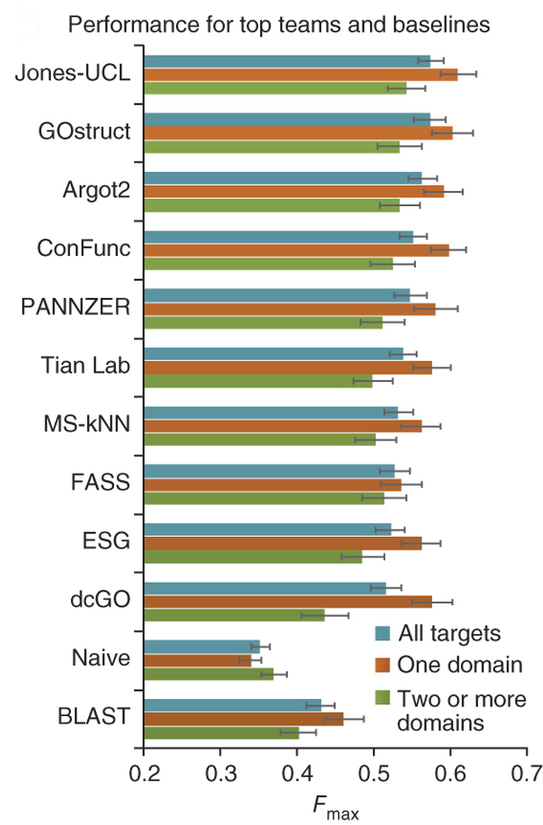
\includegraphics[height=0.65\textheight]{images/cafa_results}
    \end{column}
  \end{columns}         
\end{frame}
%% genome_scale_prediction.tex
%% Author: Leighton Pritchard
%% Copyright: James Hutton Institute
%% A brief description of functional annotation

%% trip_to_the_doctor.tex
%% Author: Leighton Pritchard
%% Copyright: James Hutton Institute
%% A brief example to demonstrate the importance of accounting for multiple-testing

% SUBSECTION: a short aside
\subsection{A visit to the doctor}

\begin{frame}
  \frametitle{A wee trip to the doctor}
  \begin{itemize}
    \item<1-> You go for a checkup, and are tested for disease $X$
    \item<1-> The test has \textbf{$\text{sensitivity}=0.95$} (predicts disease where there is disease)
    \item<1-> The test has \textbf{$\text{FPR}=0.01$} (predicts disease where there is no disease)
    \item<2-> Your test is \emph{positive}
    \item<2-> \textbf{What is the probability that you have disease $X$?}
    \begin{itemize}
      \item \textbf{0.01, 0.05, 0.50, 0.95, 0.99?}
    \end{itemize}
    \item<2-> (Audience Participation!)
  \end{itemize} 
\end{frame}

\begin{frame}
  \frametitle{A wee trip to the doctor}
  \begin{itemize}
    \item<1-> What is the probability that you have disease $X$?
    \item<1-> \textbf{Unless you know the \emph{baseline occurrence} of disease $X$, you cannot determine this.}
    \item<2-> Baseline occurrence: $f_X$
    \begin{itemize}
      \item $f_X = 0.01 \implies P(\text{disease}|\text{+ve}) = 0.490 \approx 0.5$
      \item $f_X = 0.8 \implies P(\text{disease}|\text{+ve}) = 0.997 \approx 1.0$         
    \end{itemize}
  \end{itemize} 
\end{frame}





% SUBSECTION: Genome-scale prediction
\subsection{Statistics of genome-scale prediction}
\begin{frame}
  \frametitle{Why Performance Metrics Matter\footnote{\tiny{\href{http://dx.doi.org/10.1007/978-1-62703-986-4_4}{Pritchard and Broadhurst (2014) \textit{Methods Mol. Biol.} \textbf{1127}:53-64 doi:10.1007/978-1-62703-986-4\_4}}}}
  \begin{itemize}
    \item<1-> Imagine a paper describing a predictor for protein functional class (e.g. Type III effector)
    \item<1-> The paper reports \textbf{$\text{sensitivity}=0.95$}, \textbf{$\text{FPR}=0.01$}
    \item<1-> You run the predictor on 20,000 proteins in an organism
    \item<1-> It predicts 130 members of the class. How many of them are likely to be true positives?
    \item<2-> \textit{We need a baseline level of that class ($f_X$) in the genome to determine this.}        
    \item<2-> We estimate $\approx$ 200 members in protein complement, so $f_X=0.01$
    \begin{itemize}
      \item $f_X = 0.01 \implies P(\text{class}|\text{+ve}) = 0.490 \approx 0.5$
    \end{itemize}
  \end{itemize} 
\end{frame}

\begin{frame}
  \frametitle{Bayes' Theorem}
  \begin{itemize}
    \item May seem counter-intuitive: 95\% sensitivity, 99\% specificity $\implies$ \textbf{50\% chance} of any prediction being incorrect
    \item Probability given by Bayes' Theorem
    \begin{itemize}
      \item $P(X|+) =  \frac{P(+|X) P(X)}{P(+|X) P(X) + P(+|\bar{X}) P(\bar{X})}$
    \end{itemize}
    \item This step commonly overlooked in the literature
      \begin{itemize}
        \item confirmation bias
        \item people want to see positive examples/tell a story
        \item people want to think their predictor works
      \end{itemize}
  \end{itemize} 
\end{frame}

\begin{frame}
  \frametitle{A cautionary tale\footnote{\tiny{\href{http://dx.doi.org/10.1371/journal.ppat.1000376}{Arnold \textit{et al}. (2009) \textit{PLoS Pathog.} \textbf{5}:e1000376 doi:10.1371/journal.ppat.1000376}}}}
  \begin{itemize}
    \item<1-> Paper describes \texttt{EffectiveT3}, a type III effector prediction tool
    \item<1-> Reported \textbf{sensitivity $\approx$ 0.71, FPR $\approx$ 0.15}
    \item<1-> Applied tool to 739 complete bacterial and archaeal genomes
    \item<2-> Organisms with an identifiable T3SS: 2-7\% of genome predicted to be secreted
    \item<2-> \textbf{Organisms without an identifiable T3SS (or known not to have one): 1-10\% of genome predicted to be secreted}
    \item<2-> ``\textit{The surprisingly high number of (false) positives in genomes without T3SS exceeds the expected false positive rate}''
    \item<2-> This is not a surprise, statistically.
  \end{itemize} 
\end{frame}

\begin{frame}
  \frametitle{A cautionary tale\footnote{\tiny{\href{http://dx.doi.org/10.1371/journal.ppat.1000376}{Arnold \textit{et al}. (2009) \textit{PLoS Pathog.} \textbf{5}:e1000376 doi:10.1371/journal.ppat.1000376}}}}
    Probability that an \texttt{EffectiveT3} positive prediction corresponds to a secreted protein is given by Bayes' Theorem \\[0.2cm]
    \begin{itemize}
      \item $P(X|+) =  \frac{P(+|X) P(X)}{P(+|X) P(X) + P(+|\bar{X}) P(\bar{X})}$
      \begin{itemize}
        \item $P(+|X)$ = sensitivity = 0.71
        \item $P(+|\bar{X})$ = FPR = 0.15
        \item $P(X)$ = base rate $\approx$ 0.03 $^($\footnote{\tiny{\href{http://dx.doi.org/10.1146/annurev-phyto-080508-081936}{Boch and Bonas (2010) \textit{Annu. Rev. Phytopathol.} \textbf{48}:419-436 doi:10.1146/annurev-phyto-080508-081936}}}$^)$
        \item $\implies P(X|+) \approx 0.13$
      \end{itemize}
    \end{itemize}
  \textbf{Only 13\% of predictions likely to be positive!}\\[0.1cm]
  How many predicted type III secreted proteins were there$\ldots$
\end{frame}

\begin{frame}
  \frametitle{A cautionary tale\footnote{\tiny{\href{http://dx.doi.org/10.1371/journal.ppat.1000376}{Arnold \textit{et al}. (2009) \textit{PLoS Pathog.} \textbf{5}:e1000376 doi:10.1371/journal.ppat.1000376}}}}
  \begin{center}
    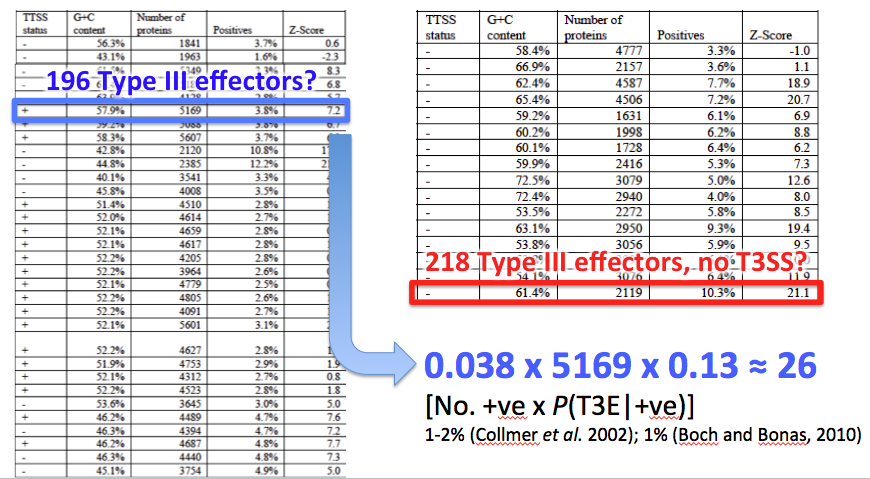
\includegraphics[height=0.65\textheight]{images/arnold_results}  
  \end{center}
\end{frame}

\begin{frame}
  \frametitle{Interpreting genome-scale predictions\footnote{\tiny{\href{http://dx.doi.org/10.1007/978-1-62703-986-4_4}{Pritchard and Broadhurst (2014) \textit{Methods Mol. Biol.} \textbf{1127}:53-64 doi:10.1007/978-1-62703-986-4\_4}}}}
  \begin{itemize}
    \item<1-> Statistics at genome-scale can be counterintuitive.
    \item<1-> \textbf{Use Bayes' Theorem!}
    \item<1-> Predictions identify groups, not individual members of the group. e.g.
    \begin{itemize}
      \item Test for airport smugglers has $P(\text{smuggler}|+) = 0.9$
      \item Test gives 100 positives
    \end{itemize}
    \item<1-> Which specific individuals are truly smugglers?
    \item<2-> The test \emph{does not} allow you to determine this - you need more evidence for each individual
    \item<2->  Same principle applies to other classifiers, (including protein functional class prediction) - watch for `cherry-picking' in publications
  \end{itemize} 
\end{frame}

%%%
% SECTION: Genome-Scale Functional Prediction
\section{Building to Metabolism}
%% building_to_metabolism.tex
%% Author: Leighton Pritchard
%% Copyright: James Hutton Institute
%% A brief introduction to orthologues, and evaluation of their prediction

% SUBSECTION: Reconstructing metabolism
\subsection{Reconstructing metabolism}

% Which methods work best
\begin{frame}
  \frametitle{Reconstructing metabolism\footnote{\tiny{Thiele and Palsson (2010) \textit{Nat. Protoc.} \textbf{5}:93-121 \href{http://dx.doi.org/10.1038/nprot.2009.203}{doi:10.1038/nprot.2009.203}}}}
  Once metabolic functional annotation has been assigned to features, we can do comparative analysis of metabolism.
  \begin{center}
      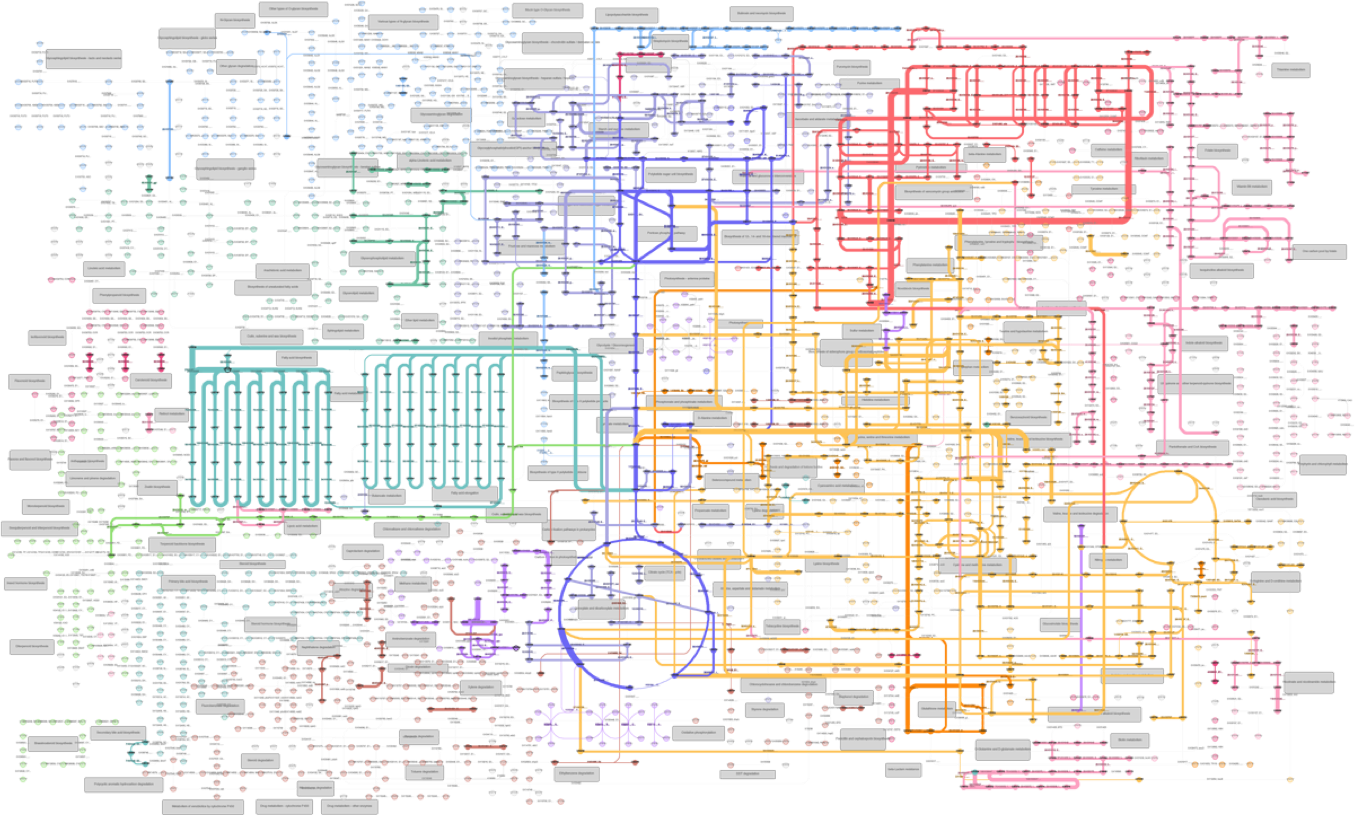
\includegraphics[width=1\textwidth]{images/dickeya_metabolism} 
  \end{center}
\end{frame}

% Which methods work best
\begin{frame}
  \frametitle{Dynamic models of metabolism\footnote{\tiny{Orth \textit{et al.} (2010) \textit{Nat. Biotech.} \textbf{28}:245-248 \href{http://dx.doi.org/10.1038/nbt.1614}{doi:10.1038/nbt.1614}}}}
  By using constraint-based models (e.g. Flux Balance Analysis), we can make these into dynamic representations of bacterial metabolism.
  \begin{itemize}
    \item Upper, lower bounds to reaction rates
    \item Define objective phenotype
    \item Calculate conditions resulting in flux
    \item \textit{in silico} knockouts
  \end{itemize}
  \begin{center}
      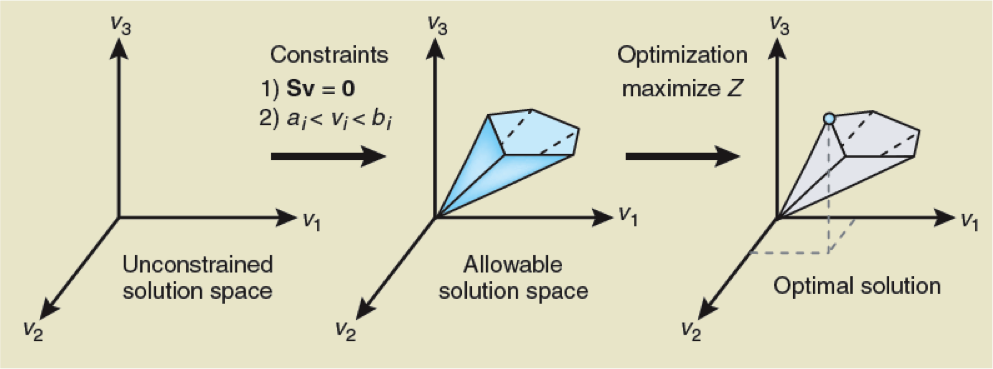
\includegraphics[width=1\textwidth]{images/fba} 
  \end{center}
\end{frame}

% Which methods work best
\begin{frame}
  \frametitle{\textit{E. coli} metabolism\footnote{\tiny{Monk \textit{et al.} (2013) \textit{Proc. Natl. Acad. Sci. USA} \textbf{110}:20338-20343 \href{http://dx.doi.org/10.1073/pnas.1307797110}{doi:10.1073/pnas.1307797110}}}}
  \textit{E. coli} has a very long history of metabolic reconstruction\footnote{\tiny{Reed and Palsson (2000) \textit{J. Bact.} \textbf{185}:2692-2699 \href{http://dx.doi.org/10.1128/JB.185.9.2692-2699.2003}{doi:10.1128/JB.185.9.2692-2699.2003}}}\\
  Recent modelling work predicts which nutrients support growth
  \begin{center}
      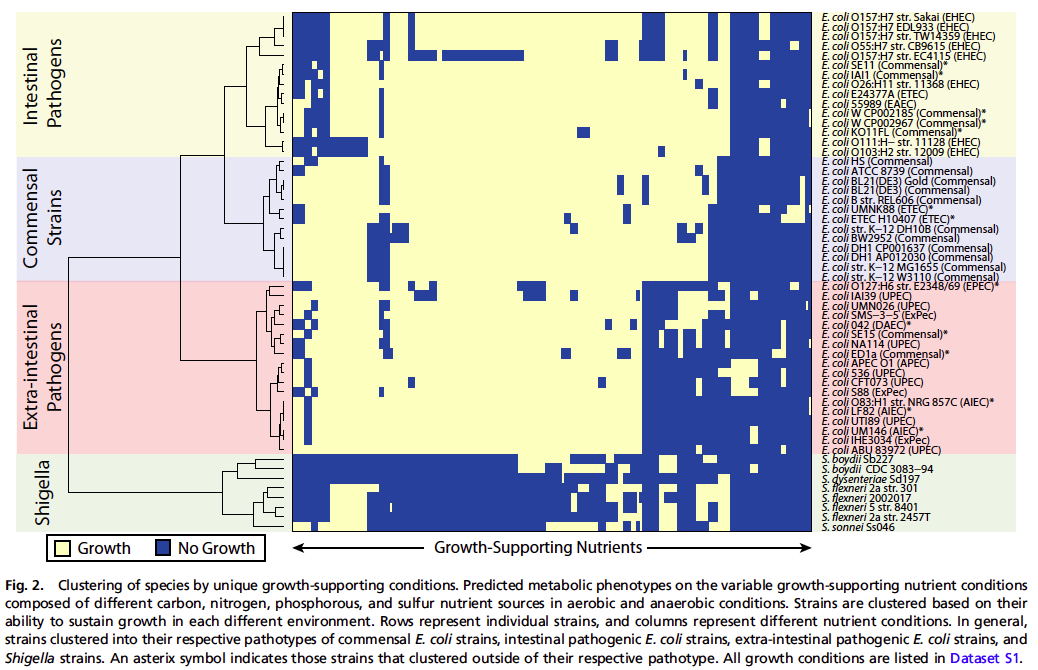
\includegraphics[width=0.85\textwidth]{images/e_coli_growth} 
  \end{center}
\end{frame}

% Which methods work best
\begin{frame}
  \frametitle{\textit{E. coli} metabolism\footnote{\tiny{Baumler \textit{et al.} (2011) \textit{BMC Syst. Biol.} \textbf{5}:182 \href{http://dx.doi.org/10.1186/1752-0509-5-182}{doi:10.1186/1752-0509-5-182}}}}
  Models are complex, and experimental validation is essential
  \begin{center}
      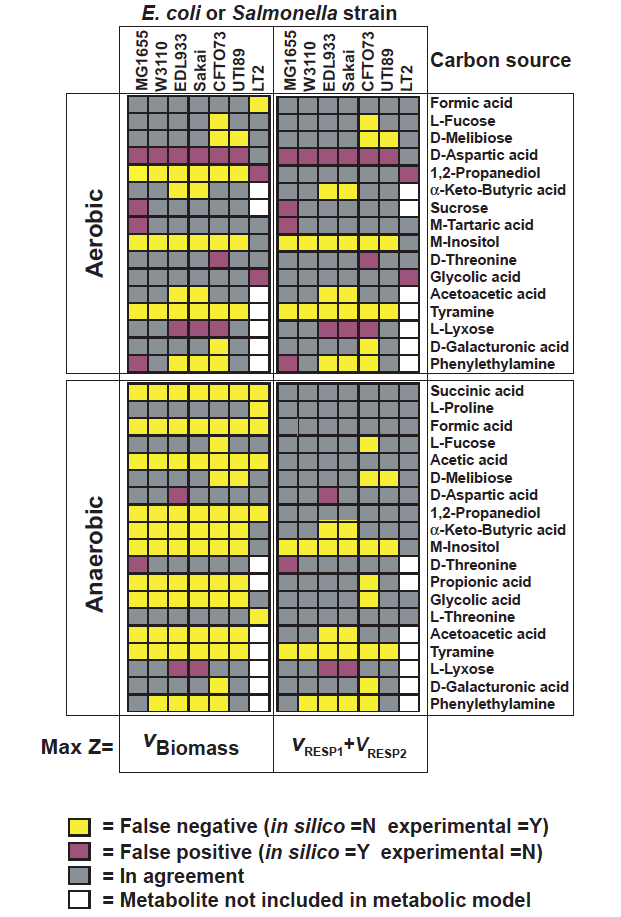
\includegraphics[width=0.4\textwidth]{images/e_coli_carbon_source} 
  \end{center}
\end{frame}

%%%
% SECTION: Things I Missed Out
%\section{Things I Missed}
%\input{sections/things_missed}

%%%
% SECTION: Conclusions
%\section{Conclusions}
%%% conclusions.tex
%% Author: Leighton Pritchard
%% Copyright: James Hutton Institute
%% A brief introduction to orthologues, and evaluation of their prediction

% Conclusions
\subsection{Things I Didn't Get To}

% Which methods work best
\begin{frame}
  \frametitle{Things I didn't get to}
  \begin{center}
      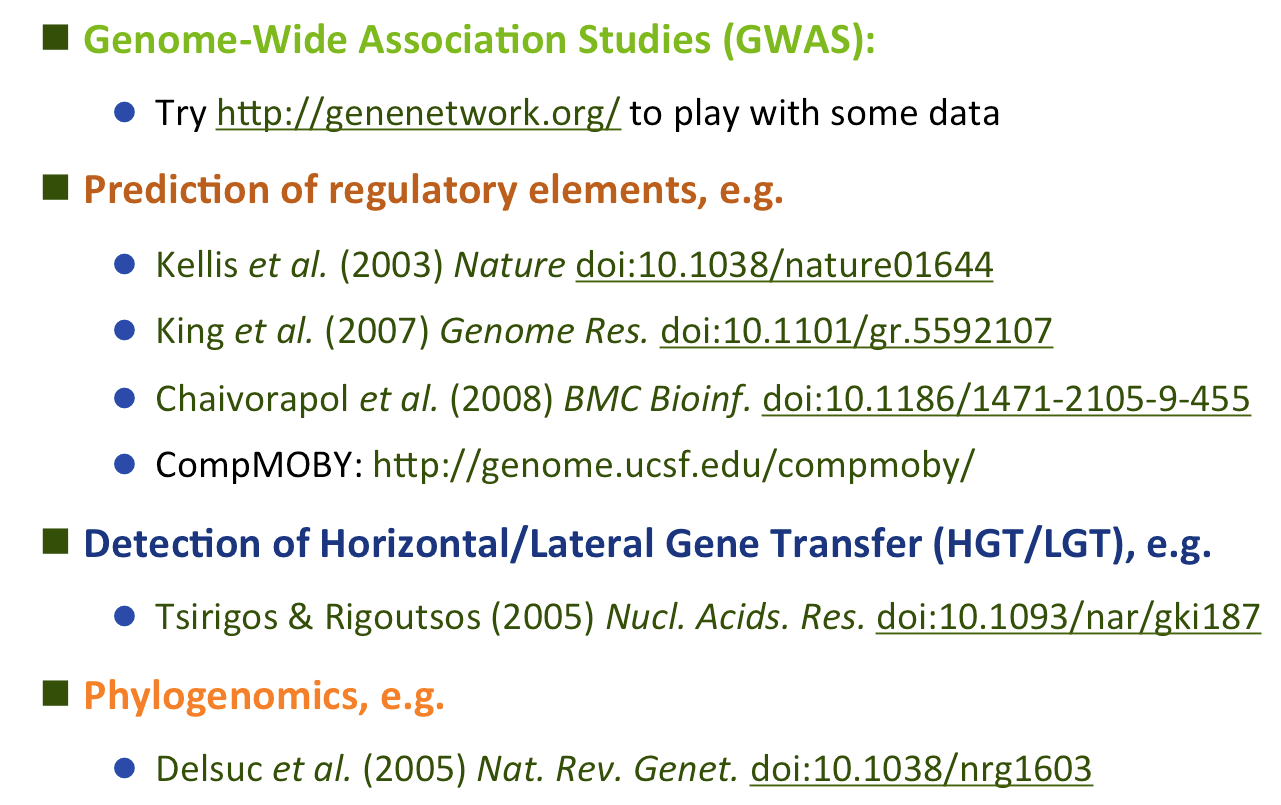
\includegraphics[width=1\textwidth]{images/didnt_get_to} 
  \end{center}
\end{frame}

% Conclusions
\subsection{Conclusions}

% Which methods work best
\begin{frame}
  \frametitle{Conclusions}
  \begin{center}
      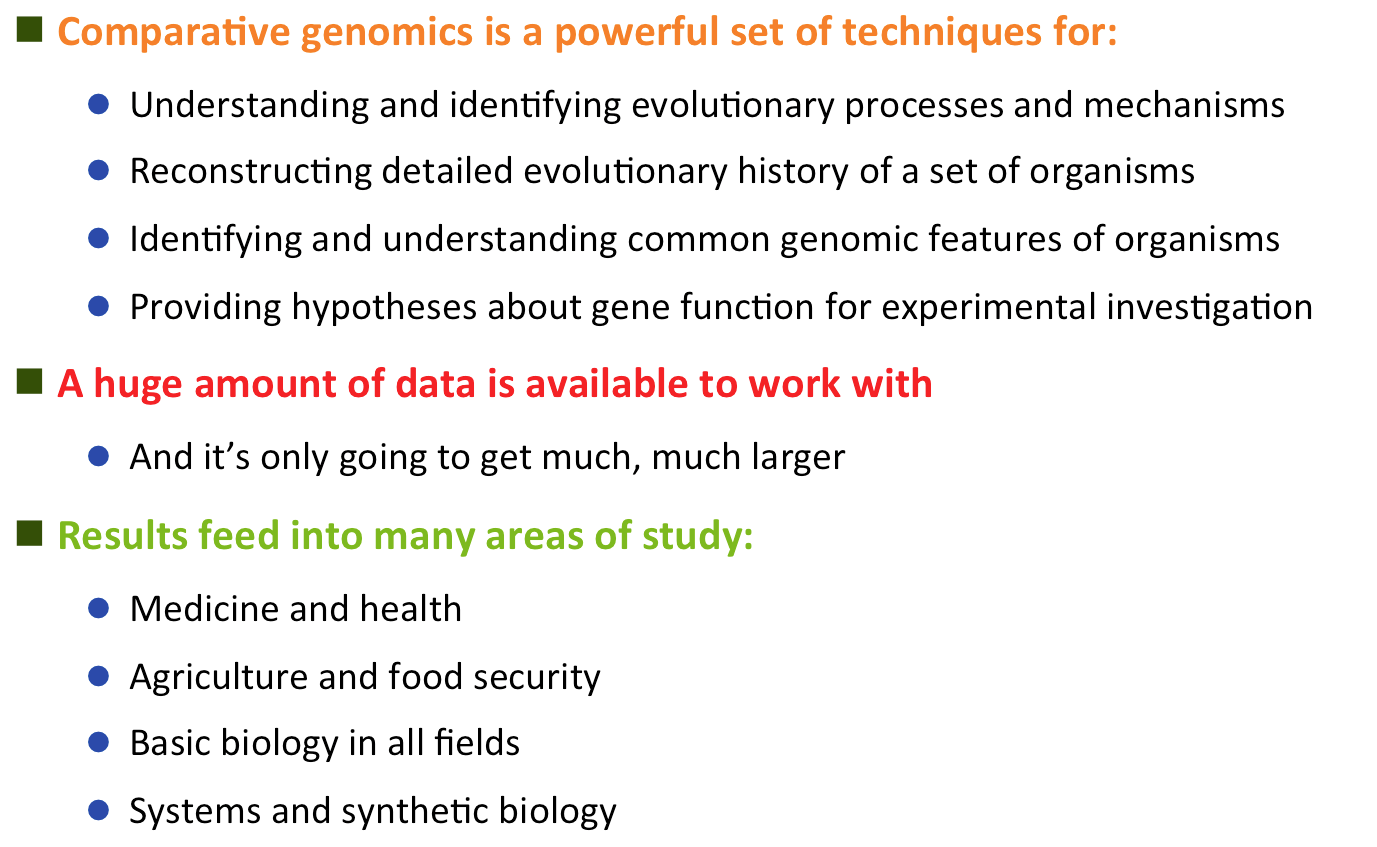
\includegraphics[width=1\textwidth]{images/conclusions1} 
  \end{center}
\end{frame}

% Which methods work best
\begin{frame}
  \frametitle{Conclusions}
  \begin{center}
      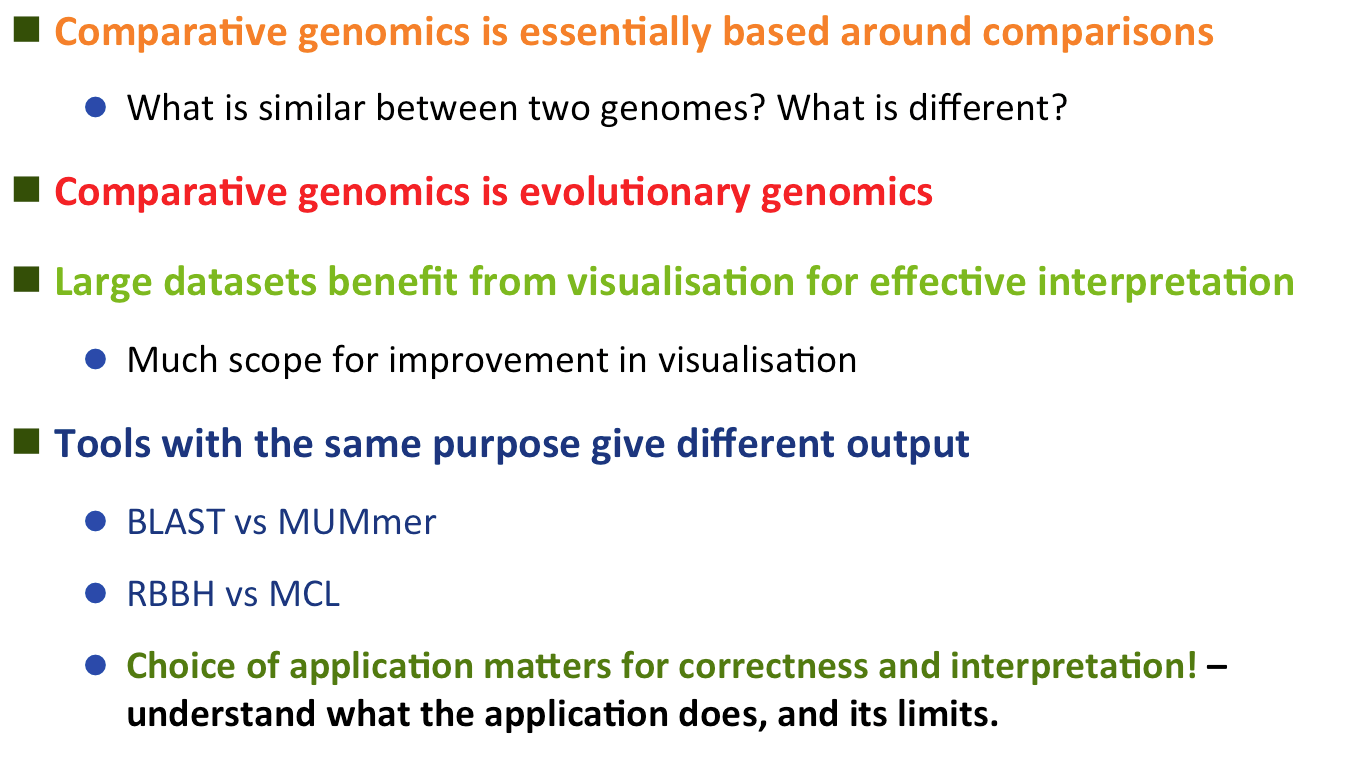
\includegraphics[width=1\textwidth]{images/conclusions2} 
  \end{center}
\end{frame}

% Which methods work best
\begin{frame}
  \frametitle{Conclusions}
  \begin{center}
      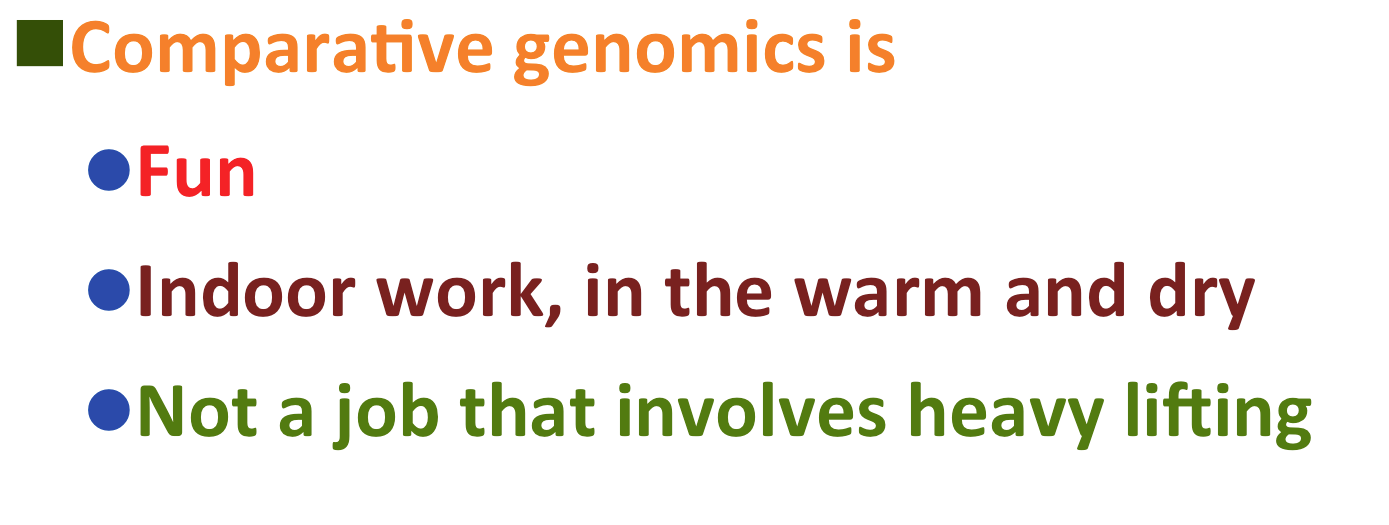
\includegraphics[width=1\textwidth]{images/conclusions3} 
  \end{center}
\end{frame}


%%%
% ACKNOWLEDGEMENTS
%\section{Acknowledgements}
%\input{sections/acknowledgements}


%%%
% LICENCE FOR REUSE
%% licence.tex
%% Author: Leighton Pritchard
%% Copyright: James Hutton Institute
%% These slides describe the licence for reuse of these slides and
%% materials

%
\begin{frame}
  \frametitle{Licence: CC-BY-SA}
  By: Leighton Pritchard \\[0.5cm]
  This presentation is licensed under the Creative Commons Attribution ShareAlike license \\
  \href{https://creativecommons.org/licenses/by-sa/4.0/}{https://creativecommons.org/licenses/by-sa/4.0/}
\end{frame}

% etc
\end{document}